\documentclass{article}
\usepackage{amsmath}
\usepackage{amssymb}
\usepackage{a4wide}
\usepackage{graphicx}
\usepackage{float}      

\title{Stat 17 Week 6\\Continuous Distributions}
\author{Xiao Zhang}
\date{Febuary 2026}

\begin{document}

\maketitle

\section*{Continuous Distributions \& Standard Normal}

\paragraph{Empirical Rule (68–95–99.7 Rule)}

\begin{itemize}
    \item Applies to bell-shaped (approximately normal) distributions
    \item About 68\% of data fall within $\mu \pm 1\sigma$
    \item About 95\% of data fall within $\mu \pm 2\sigma$
    \item About 99.7\% of data fall within $\mu \pm 3\sigma$
    \item Beyond 3 standard deviations:
    \begin{itemize}
        \item Total outside area $\approx 0.3\%$
        \item Each tail $\approx 0.15\%$
    \end{itemize}
\end{itemize}


\begin{figure}[ht]
    \centering
    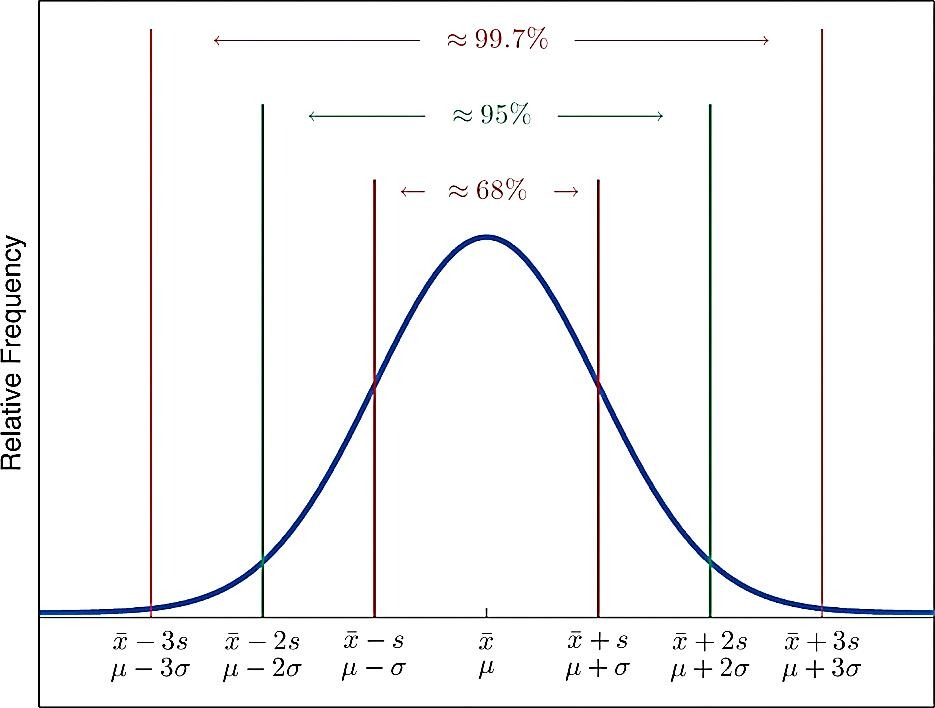
\includegraphics[width=0.85\textwidth]{empirical_rule.jpg}
    \caption{Visualization of the Empirical Rule}
\end{figure}



\paragraph{Uniform Distribution}

\begin{itemize}
    \item If $X \sim U(a,b)$, then probability is based on interval length
    \[
    P(c < X < d) = \frac{d-c}{b-a}
    \]
    \item All values in $(a,b)$ are equally likely
    \item Graph is a rectangle (constant density)
\end{itemize}

\paragraph{Normal Distribution}

\begin{itemize}
    \item Bell-shaped and symmetric
    \item Completely determined by:
    \begin{itemize}
        \item Mean $\mu$
        \item Standard deviation $\sigma$
    \end{itemize}
    \item Standard normal distribution:
    \[
    Z \sim N(0,1)
    \]
\end{itemize}

\paragraph{Z-Score}

\begin{itemize}
    \item Standardization formula:
    \[
    z = \frac{x - \mu}{\sigma}
    \]
    \item Measures how many standard deviations a value is from the mean
    \item Used to compare relative performance
    \item More unusual values have larger $|z|$
\end{itemize}


\paragraph{Converting to Standard Normal}

\begin{itemize}
    \item If $X \sim N(\mu, \sigma)$, convert using:
    \[
    Z = \frac{X - \mu}{\sigma}
    \]
    \item After converting, use z-table
\end{itemize}

\paragraph{Finding Probabilities}

\begin{itemize}
    \item Left tail:
    \[
    P(X < a)
    \]
    \item Right tail:
    \[
    P(X > a) = 1 - P(X < a)
    \]
    \item Between two values:
    \[
    P(a < X < b) = P(z_1 < Z < z_2)
    \]
\end{itemize}

\paragraph{Percentiles}

\begin{itemize}
    \item To find a percentile:
    \begin{enumerate}
        \item Find corresponding z-score from table
        \item Convert back:
        \[
        x = \mu + z\sigma
        \]
    \end{enumerate}
\end{itemize}

\paragraph{Common Z-Values}

\begin{itemize}
    \item 95\% confidence level: $z = 1.96$
    \item Middle 99\%: $z = \pm 2.575$
    \item 90th percentile: $z = 1.28$
    \item 75th percentile: $z = 0.67$
\end{itemize}

\paragraph{Two Types of Z-Tables}

\begin{itemize}
    \item Table A: $T(z) = P(0 < Z < z)$
    \item Table B: $\Phi(z) = P(Z < z)$
    \item Relationship (for $z > 0$):
    \[
    \Phi(z) = 0.5 + T(z)
    \]
\end{itemize}

\end{document}
